\chapter{A New Breed of Counting}
We are going to encounter a new breed of Combinitorics now onward where we are not so 
interested in counting in the ways to do something but in proving that there exists 
some way of doing something or more often, there exists no way of doing something. 
We'll now look at tiling's and coloring and expected values and betting and games and a lot, 
lot more. While this section begins our foray into the more robust real life uses of Combi, 
it is still relevant to Olympiads. A beginning example could be:\\
\begin{example}
    (RMO 2023) Consider a set of $16$ points arranged in $4 \times 4$ square grid formation. Prove that if any $7$ of these points are coloured blue, then there exists an isosceles right-angled triangle whose vertices are all blue.
\end{example}
\begin{proof}
    Probably the hardest problem on the test.\\
    Fun story, I actually gave the test when this question came. Overconfident in my combi, I messed it up pretty bad as I created a non-existent counter example. I'll leave the details to your imagination.\\
    The solution proceeds by observing the possible isosceles triangles.\\
    \begin{figure}{H}
        \centering
        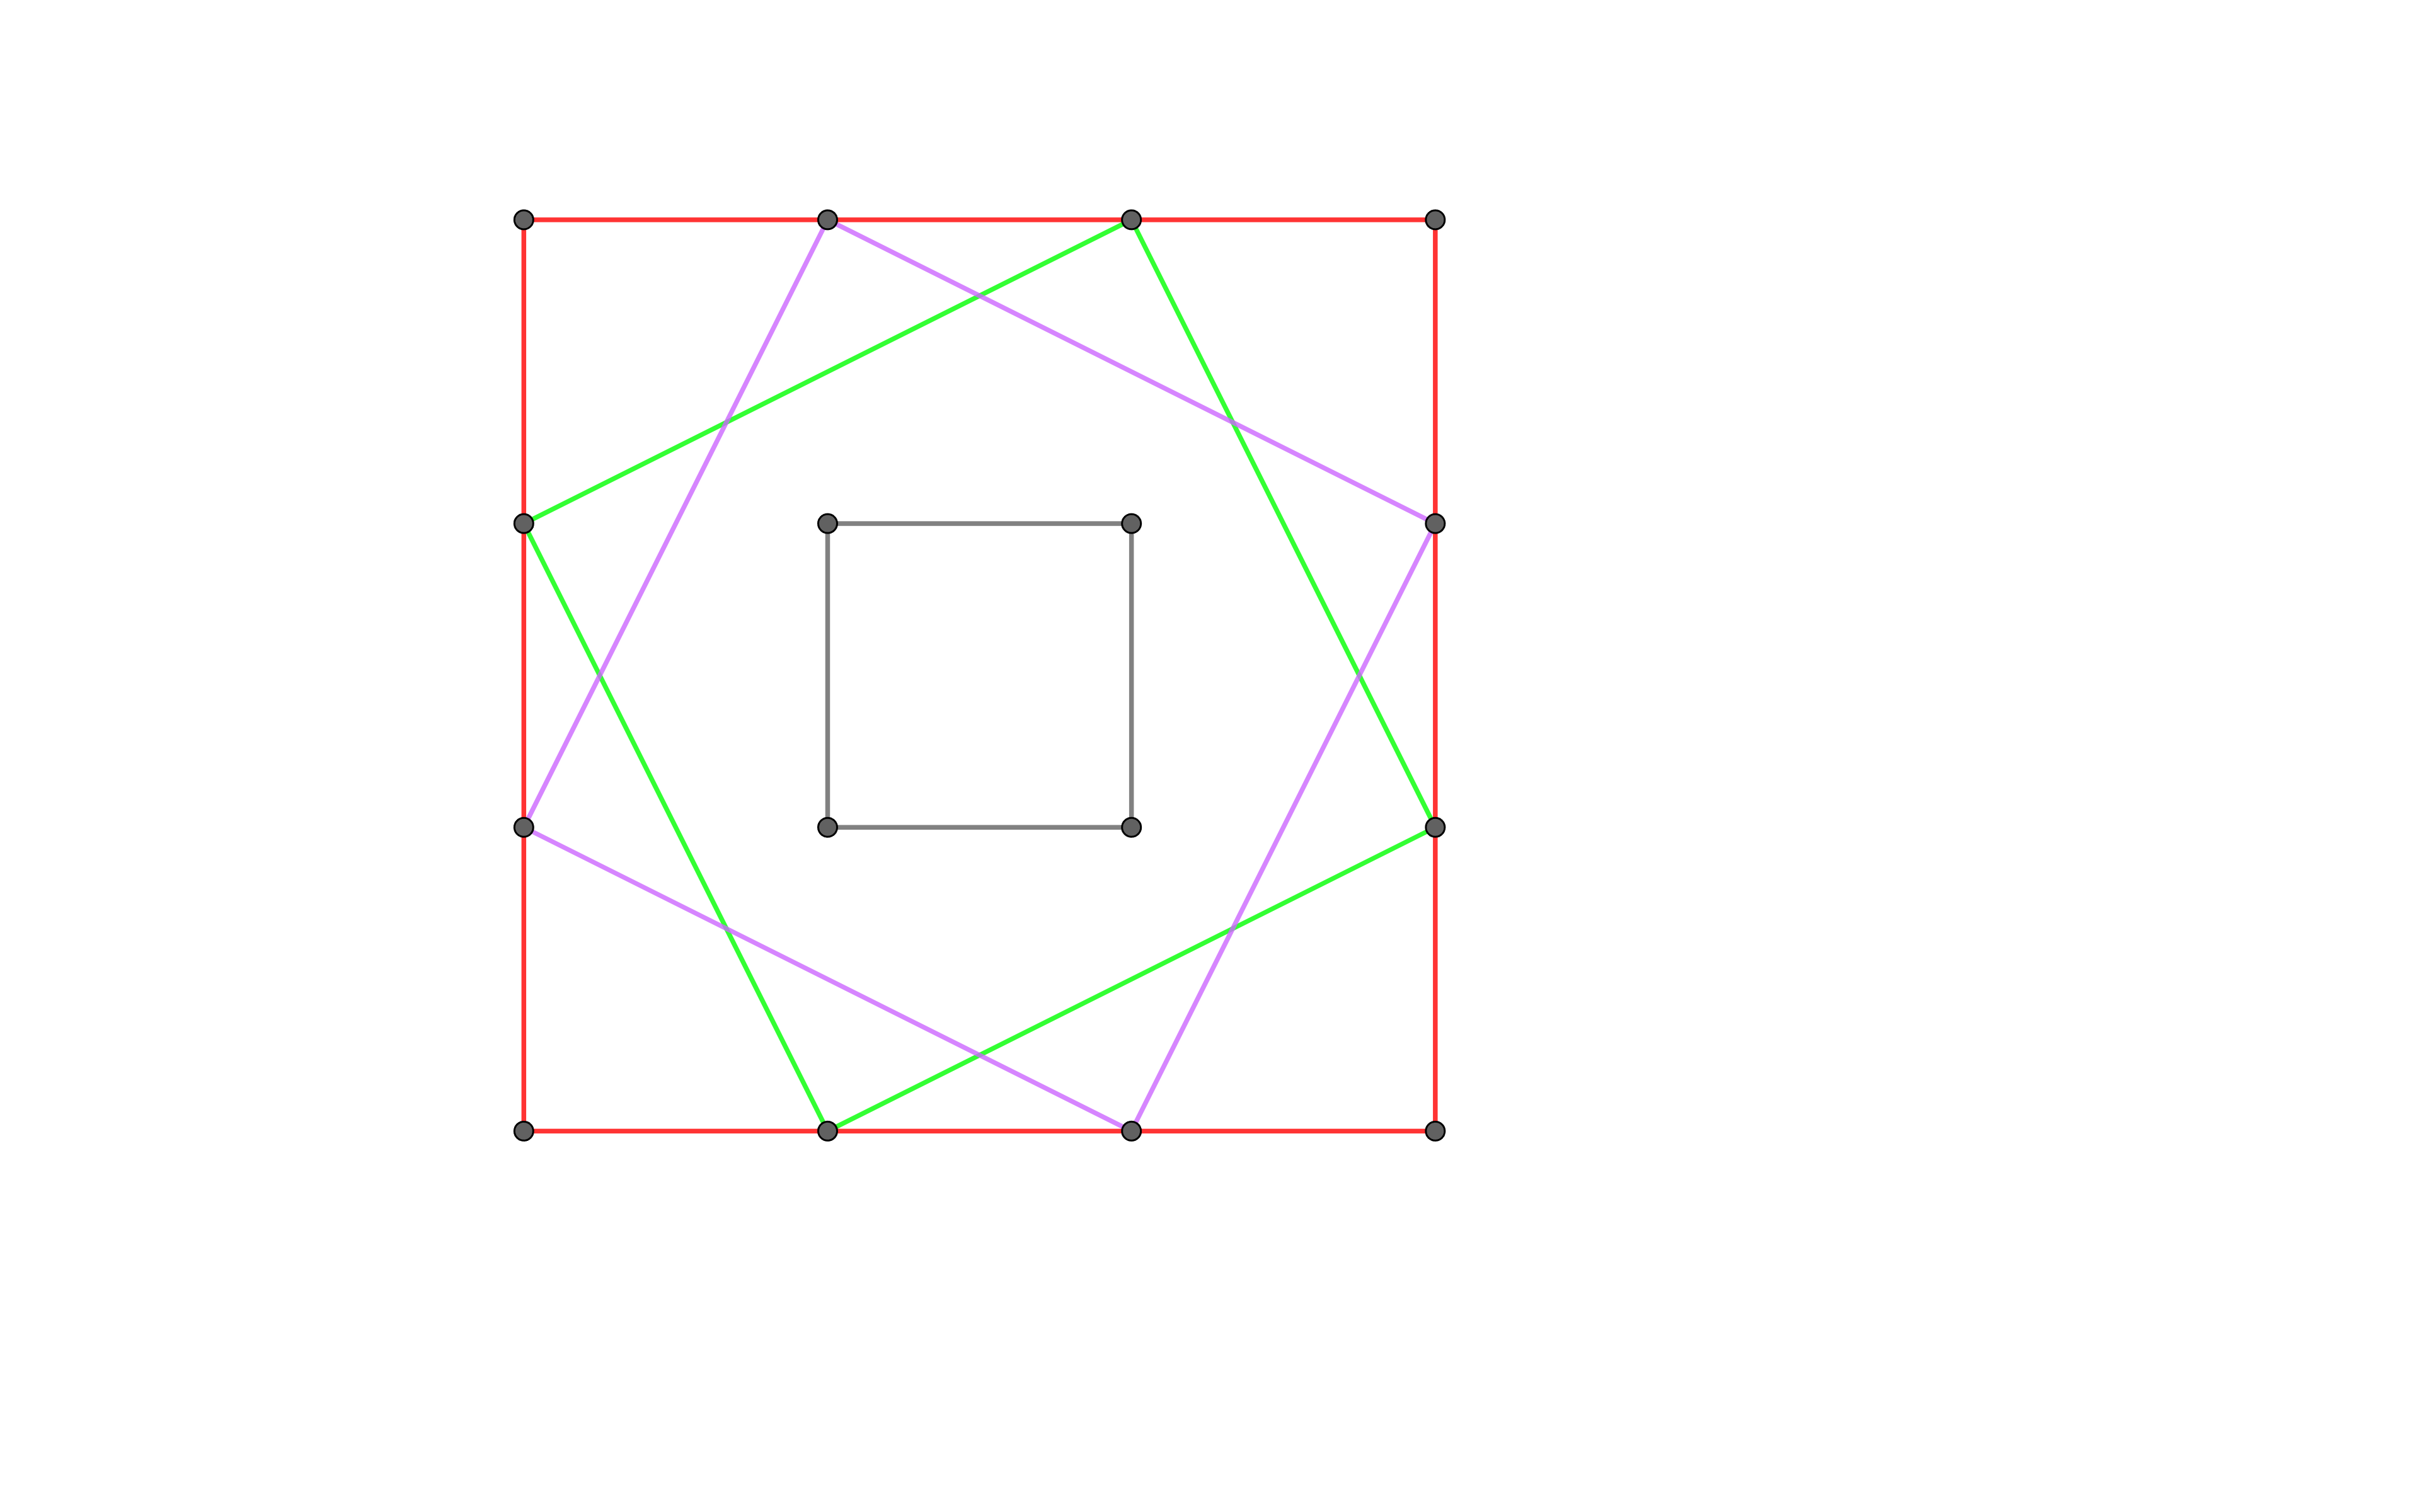
\includegraphics[width=0.5\linewidth]{Photos/RMO6 2023.png}
        
    \end{figure}
    We need to see that either three points lie on the vertices of a square or $2$ on the vertices of the surrounding three squares and $1$ on the center.\\
    We therefore have at most $2$ points on the outside squares, which is $2*3=6$. But as $7$ points are colored, either a square has more than $2$ vertices colored or the center square has a colored vertex.\\
    Thus, the stated claim is true.\\
\end{proof}
Let's get started with the most complex simple thing!
\section{Pigeon Hole Principle}
This PHP while very powerful, seems stupid when heard/read for the first time:
\begin{theorem}
    [Pigeon hole principle]
    Consider a flock of pigeons nestled in a set of $n$ pigeonholes. If there are $n$ pigeons, then it is possible for all of the pigeons to rest happily in separate pigeonholes. However, if at least one more pigeon arrives, making a total of more than $n$ pigeons, then at least one of the pigeonholes, inevitably, will end up with more than one pigeon.\\
    In particular, if $k$ pigeons are put into $n$ holes, there are at least $\lceil \frac{k}{n} \rceil$ in one of the holes.
\end{theorem}
While PHP may seem pointless, even offensively funny to some, a correct choice of pigeons and holes can simplify quite a lot of problems. It was first used by Dirichlet and is therefore also called the Dirichlet principle. Here is an IMO problem to show PHP's power:\\
\begin{example}
    (IMO/1 1972) Prove that from a set of ten distinct two-digit numbers (in the decimal system), it is possible to select two disjoint subsets whose members have the same sum?
\end{example}
\begin{proof}
    Let the number of subsets be the pigeons and the possible sums be the holes. \\
    We have $2^{10} -2 =1022$ subsets and $90+91+92 \dots +99 - 10 + 1$ possible sums. As $100*10=1000 \leq 1022$, the pigeons are far less than the holes. Hence, two are sure to share the hole and hence, we will always have two disjoint subsets whose members have the same sum.
\end{proof}
You have already used PHP before in a much simpler form to answer riddles like: "You have $14$ brown socks, $14$ blue socks and $14$ black socks in your sock drawer. How many socks must you remove (without looking to be sure) to have a matched pair?"\\
We didn't give it a name then as the uses were obvious. As they become more complex, a name was given to the idea.\\
PHP, while simple,  can be extended to real analysis and other branches of mathematics in the following form:\\
\begin{theorem}
[Infinite PHP]
Given an infinite pigeons, if they are put into finite pigeon holes, there is at least one pigeon hole with infinite pigeons.
\end{theorem}
We can use this to prove something of the form:\\
\begin{example}
    A $100\times100$ board is divided into unit squares. In every square there is an arrow that points up, down, left or right. The board square is surrounded by a wall, except for the right side of the top right corner square. An insect is placed in one of the squares. Each second, the insect moves one unit in the direction of the arrow in its square. When the insect moves, the arrow of the square it was in moves $90$ degrees clockwise. If the indicated movement cannot be done, the insect does not move that second, but the arrow in its squares does move. Is it possible that the insect never leaves the board?
\end{example}
\begin{proof}
    Let's assume to the contrary that there is some arrangement such that the insect is trapped.\\
    In this case, it will make infinite moves. As there are only $100^2$ pigeon holes, the insect visits some square infinite time.\\
    As the arrows keep changing, it also visits the neighbouring squares infinite times.\\
    By the same logic, it visits all the squares infinite times. Hence, it visits the top right square infinite times, which would mean it is not trapped.\\
    This is a contradiction, hence our initial assumption is false. There exists no such arrangement such that the insect is trapped.\\
    Hence, proved.
\end{proof}
Before we move ahead, here is a classic PHP question for you to try which we can also do using Extremal principle(later in this chapter).\\
\begin{example}
    There are $17$ points inside an equilateral triangle with side lengths $1$. Prove there are at least
two points within distance $\frac{1}{4}$ of each other.\\
Hint: Try dividing the triangle in equal parts.
\end{example}
\section{Expected Value and Probabilistic Method}
The probabilistic method refers to proving the existence of some element in a set by showing the probability of its existence is non-zero.\\
Cutting out the jagron, let's say I have bag of candy. How do you prove that I have a Kit-Kat in the bag? You either keep on removing chocolates till you get a Kit-Kat, or through some tricks you prove that the probability of drawing a Kit-Kat is not zero.\\
Another allegory would be thinking of it like rolling a dice. If you roll a regular six-sided dice, there's a chance of getting any number from 1 to 6. The probabilistic method is a bit like saying, "Hey, there's a chance, maybe a small one, but it's not zero, that I'll get a 6." So, you can be pretty confident that a 6 exists on that dice, even if you haven't seen it yet.\\
This was explained thrice to provide the motivation to define the following.
\begin{defination}
[Expected Value]
For a random variable $X$,  $\E{x}=\sum {x_i \cdot P(x_i)}$ where $x_i$ are the possible values of X and $P(x_i)$ is the probability of the value being $x_i$
\end{defination}
For example for a dice, let $X$ be the number on the die. Then $\E{x}=\frac{1}{6}1+\frac{1}{6}2+\dots+\frac{1}{6}6 =3.5$.\\
What this tells us is that if we roll a dice, we expect the value to be $3.5$. While $3.5$ is not a number on the dice, over a lot of throws this is the average of roll of a dice.\\
We now define the most important theorem of the probabilistic method
\begin{theorem}
[Linearity of Expectations] $\E{X_1+X_2+X_3+\dots +X_n}=\E{x_1}+\E{x_2}+\dots +\E{x_n}$\\
\end{theorem}
This is obvious when the variables are independent. However, the beauty of this theorem is based on the fact that that even if they are not independent, this still stands. The proof has been omitted as it can be made using a incidence matrices and then summing up. You will end up with a ugly summation which will mean the same as above. Google it if you are curious!\\
Let's see a classic example\\
\begin{example}
[HMMT 2006] At a nursery, $2006$ babies sit in a circle. Suddenly, each baby randomly pokes either the baby to its left or to its right. What is the expected value of the number of unpoked babies?
\end{example}
\begin{proof}
    [Solution]
Let me introduce you to the most classy way of using the probabilistic method. We define a variable $P_n$ for the $n^{th}$ baby in the circle where $P=0$ if the baby is poked and $P=1$ if it is unpoked.\\
The probability of a baby being unpoked is $\frac{1}{4}$. Which means expected value of $P_n$ is $\frac{1}{4}$ which means using Linearity of Expectations(LOE) we can say that $\E{\text{Number of unpoked babies}}=\E{P_1+P_2+\dots+P_{2006}}=\E{P_1}+\dots+\E{P_{2006}}=\frac{2006}{4}$\\
\end{proof}
We can also have questions which while can be done using the probabilistic method, also have simpler solutions.
\begin{example}
(AMC 10 2021) Five balls are arranged around a circle. Chris chooses two adjacent balls at random and interchanges them. Then Silva does the same, with her choice of adjacent balls to interchange being independent of Chris’s. What is the expected number of balls that occupy their original positions after these two successive transpositions?
\end{example}
\begin{proof}
    [Solution]
We can also do this by the definition of expected value. Without loss of generality, let's say Chris interchanged the first ball with the second ball.\\
Silva can now interchange either the same two($\frac{1}{5}$ probability) which leaves us with $5$ balls in the original position.\\
Silva can interchange one of the balls Chris switched with another neighbour($\frac{2}{5}$ probability) which leaves $2$ balls in the original position.\\
Silva can interchange two entirely new balls(\frac{2}{5} probability) which leaves $1$ ball in the original position.\\
This means the expected value is $\frac{1}{5}*5+\frac{2}{5}*2+\frac{2}{5}*1=1+0.8+0.4=2.2$\\
If we want to use probabilistic method, we can define a variable $P$ for every ball which is $0$ if the ball is not on its original position and $1$ if it is.\\
So the Expected value of $P$ is the sum of the probability of the ball never being switched and it being switched twice.\\
$\therefore \E{P}=(\frac{3}{5})^2+\frac{2}{5}\cdot\frac{1}{5}=\frac{11}{25}$\\
As we have $5$ balls, Using LOE, the expected number of balls in the original position are $\frac{11}{25}*5=\frac{11}{5}=2.2$
\end{proof}
To the contrary of the last example, here is one which cannot be solved neatly without LOE.\\
\begin{example}
    (Putnam 2014, A4)Suppose $X$ is a random variable that takes on only non-negative integer values, with $\E{X}=1$, $\E{X^2} = 2$, and $\E{X^3} = 5$. Determine the smallest possible value of the probability of the event $X=0$.
\end{example}
\begin{proof}
    We need to realize that given expected value of $x, x^2$ and $x^3$, we can find the expected value of any polynomial with degree $3$ or less courtesy linearity of expectations.\\
    This means we know the expected value of $f(x)=(x-1)(x-2)(x-3)=x^3-6x^2+11x-6$ which is $0$ for $1,2,3$.\\
    $\E{f(x)}=5-6*2+11*1-6=5-12+11-6=-2$\\
    We need to now notice that $f(0)=-6$ and $f(x)>0$ for all $x>3$. So as the probability of $x>3$ increases, probability of $x=0$ also increases.\\
    For the minimum case, let probability of $x=0$ be $p$ and probability of $x=1,2,3$ be $1-p$.\\
    This means $-6p=-2 \iff p=\frac{1}{3}$.\\
    We can construct probability for $1,2,3$ to satisfy the equations. That is left for you to try yourself.
\end{proof}
Before moving onto some other applications of this method, I'll give a brief view of how it ends up used in active research. Also I'll introduce a powerful graph theory theorem at the same time, and show off another way of setting the variable. One stone, three pigeons\\
\begin{theorem}
[Turan's Theorem] For $G = (V, E)$. Let an independent set be a set of vertices such that no two are adjacent. $G$ contains an independent set of size at least $\sum_{v \in V}\frac{1}{d(v)+1}$
\end{theorem}
\begin{proof}
We'll permute all the vertices in a line. Let's define a variable $S$ as the number of vertices such that a vertex in the permutation lies before all vertices adjacent to it. The expected value of this is obviously the expected size of an independent set.\\
Let another variable $P$ be $1$ if all neighbours of a vertex are after it in the permutation, and $0$ otherwise. Using LOE, we can say that $\E{S}=\sum_{v \in V} \E{P_v}$.\\
We need to note that for any vertex $v$, it had $d(v)$ adjacent vertices. Only one of them, among the vertex and its neighbours, has all its neighbours after it. This means that the probability of $P_v$ being $1$ is $\frac{1}{d(v)+1}$ which means $\E{P_v}=\frac{1}{d(v)+1}$\\
Thus, expected size of independent set $\E{S}=\sum_{v \in V}\frac{1}{d(v)+1}$
\end{proof}
We will also prove the same using Extremal principal later.\\

\begin{xcb}{Exercises}
    \begin{enumerate}
\item (AMC 10 2006) A player pays $5$ dollars to play a game. A die is rolled. If the number on the die is odd, the game is lost. If the number on the die is even, the die is rolled again. In this case the player wins if the second number matches the first and loses otherwise. How much should the player win if the game is fair? (In a fair game the probability of winning times the amount won is what the player should pay.)
\item(AMC 12) A school has 100 students and 5 teachers. In the first period, each student is taking one class, and each teacher is teaching one class. The enrollments in the classes are 50, 20, 20, 5, and 5. Let t be the average value obtained if a teacher is picked at random and the number of students in their class is noted. Let s be the average value obtained if a student was picked at random and the number of students in their class, including the student, is noted. What is $t-s$?
\item (OMM 1998)The sides and diagonals of a regular octagon are colored black or red. Show that there are at least $7$ monochromatic triangles with vertices in the vertices of the octagon.
\item  Let $F_n$ be the $n^{th}$ Fibonacci numbers. Show that for some $n \geq 1$, $F_n$ ends with 2023 zeros.
\item Let $S$ be a subset of ${1, 2, 3, . . . , 2n}$ with $n + 1$ elements. Show that there are two elements in $S$ which are relatively prime.
\item (continuing of the above question) Show that there are two elements in $S$, one divisible by the other
\item At a party, certain pairs of individuals have shaken hands. Prove that there exist two persons who have shaken the same number of hands
\item Given $7$ lines on the plane, prove that two of them form an angle less than $26^{\circ}$
\item A chess grandmaster has $77$ days to prepare for a tournament. He wants to play at least one game per day, but not more than 132 games in total. Prove that there is a sequence of successive days on which he plays exactly 21 games in total.
\item (Canada 2004, edited) Let $T$ be the set of all positive integer divisors of $2023^{100}$. What is the largest possible number of elements that a subset S of T can have if no element of S is an integer multiple of any other element of S?
\item Show that there is some $n$ for which $111 \dots 111$ (with $n$ ones) is divisible by $2023$
\item (IMO/4 1964)Seventeen people correspond by mail with one another - each one with all the rest. In their letters only three different topics are discussed. Each pair of correspondents deals with only one of these topics. Prove that there are at least three people who write to each other about the same topic.
\item Prove that the decimal representation of any irrational number has at least two digits appearing
infinitely often
\item (IMO/4 1985) Given a set $M$ of $1985$ distinct positive integers, none of which has a prime divisor greater than $23$, prove that $M$ contains a subset of $4$ elements whose product is the $4$th power of an integer.
\item  Prove that among any $2m + 1$ distinct integers of absolute value less than or equal to $2m - 1$, there are three whose sum is zero.(Although can be solved using PHP, there is a much simpler way out)
\item (Putnam/A2 2002)Given any five points on a sphere, show that some four of them must lie on a closed hemisphere.
\item  Given nine points inside the unit square, prove that some three of them form a triangle whose area does not exceed $\frac{1}{8}$.
    \end{enumerate}
\end{xcb}